\documentclass{beamer}
\usepackage[utf8]{inputenc}

\usetheme{Madrid}
\usecolortheme{default}
\usepackage{amsmath,amssymb,amsfonts,amsthm}
\usepackage{txfonts}
\usepackage{tkz-euclide}
\usepackage{listings}
\usepackage{adjustbox}
\usepackage{array}
\usepackage{tabularx}
\usepackage{gvv}
\usepackage{lmodern}
\usepackage{circuitikz}
\usepackage{tikz}
\usepackage{graphicx}

\setbeamertemplate{page number in head/foot}[totalframenumber]

\usepackage{tcolorbox}
\tcbuselibrary{minted,breakable,xparse,skins}



\definecolor{bg}{gray}{0.95}
\DeclareTCBListing{mintedbox}{O{}m!O{}}{%
  breakable=true,
  listing engine=minted,
  listing only,
  minted language=#2,
  minted style=default,
  minted options={%
    linenos,
    gobble=0,
    breaklines=true,
    breakafter=,,
    fontsize=\small,
    numbersep=8pt,
    #1},
  boxsep=0pt,
  left skip=0pt,
  right skip=0pt,
  left=25pt,
  right=0pt,
  top=3pt,
  bottom=3pt,
  arc=5pt,
  leftrule=0pt,
  rightrule=0pt,
  bottomrule=2pt,

  colback=bg,
  colframe=orange!70,
  enhanced,
  overlay={%
    \begin{tcbclipinterior}
    \fill[orange!20!white] (frame.south west) rectangle ([xshift=20pt]frame.north west);
    \end{tcbclipinterior}},
  #3,
}
\lstset{
    language=C,
    basicstyle=\ttfamily\small,
    keywordstyle=\color{blue},
    stringstyle=\color{orange},
    commentstyle=\color{green!60!black},
    numbers=left,
    numberstyle=\tiny\color{gray},
    breaklines=true,
    showstringspaces=false,
}
%------------------------------------------------------------
%This block of code defines the information to appear in the
%Title page
\title %optional
{4.10.13}
\date{September  2025}
%\subtitle{A short story}

\author % (optional)
{BEERAM MADHURI - EE25BTECH11012}



\begin{document}


\frame{\titlepage}
\begin{frame}{Question}
Find the equation of the plane passing through the line of intersection of the planes 
$\vec{r} \cdot (\hat{i} + \hat{j} + \hat{k}) = 1$ and $\vec{r} \cdot (2\hat{i} + 3\hat{j} - \hat{k}) + 4 = 0$ and parallel to the $X$ axis.

\end{frame}
 
\begin{frame}{given data}
 let P1 and P2 be the plane equations whose normals are:
\begin{table}[h!]
    \centering
    \begin{tabular}{|c|c|}
\hline
\textbf{Name} & \textbf{Value} \\
\hline
Circle & $\vec{x}^\top\vec{x} - a^2 = 0$ \\
\hline
Line & $\vec{x} = \myvec{\tfrac{a}{\sqrt{2}} \\ 0} + \kappa\myvec{0 \\ 1}$ \\
\hline
\end{tabular}

    \caption{4.10.13}
    \label{table 4.10.13}
\end{table}
\end{frame}
\begin{frame}
Given equations of planes are:-
\begin{align}
P_1: \quad \vec{r}^\top \begin{pmatrix} 1 \\ 1 \\ 1 \end{pmatrix} = 1\\
P_2: \quad \vec{r}^\top \begin{pmatrix} 2 \\ 3 \\ -4 \end{pmatrix} = -4
\end{align}
\end{frame}
\begin{frame}{solution}
    \frametitle{finding the equation of plane:}
expressing the plane equations in matrix form:-
\begin{align}
\begin{bmatrix}1 & 1 & 1 & | & 1 \\2 & 3 & -4 & | & -4\end{bmatrix}
\end{align}
Using row reductions:
\begin{align}
R_2 \rightarrow R_2 - 2R_1\\
\begin{bmatrix}1 & 1 & 1 & | & 1 \\0 & 1 & -3 & | & -6\end{bmatrix}\\
\therefore \text{equation of planes:}\\
\vec{r}^\top \begin{pmatrix} 1 \\ 1 \\ 1 \end{pmatrix} = 1\\
\vec{r}^\top \begin{pmatrix} 0 \\ 1 \\ -3 \end{pmatrix} = -6
\end{align}
\end{frame}
\begin{frame}
Solving the equations to find the line of intersection of planes\\
\begin{align}
\vec{r}(\lambda) = \begin{pmatrix}0 \\-\frac{3}{4} \\\frac{7}{6}\end{pmatrix} + \lambda \begin{pmatrix}1 \\-3/4 \\-1/6\end{pmatrix}
\end{align}\\
\text{normal to plane is orthogonal to the line and x-axis}
\begin{align}
\vec{n}^\top \vec{e}_1 = 0\\
\vec{n}^\top \vec{n}_1 = 0
\end{align}
\begin{align}
where,
\end{align}
\begin{align}
\vec{e}_1 = \begin{pmatrix} 1 \\ 0 \\ 0 \end{pmatrix}\\ \vec{n}_1 = \begin{pmatrix} 1 \\ -3/4 \\ -1/6 \end{pmatrix}
\end{align}
\end{frame}
\begin{frame}
\text{Solving using row reductions:-}
\begin{align}
\begin{bmatrix}1 & 0 & 0 & | & 0 \\4 & -3 & -1 & | & 0\end{bmatrix}
\end{align}
\begin{align}
R_2 \rightarrow R_2 - 4R_1
\end{align}
\begin{align}
\begin{bmatrix}1 & 0 & 0 & | & 0 \\0 & -3 & -1 & | & 0\end{bmatrix}
\end{align}
\end{frame}
\begin{frame}
\text{plane equation using normal and a point on the line:}
\begin{align}
\vec{n}^\top (\vec{r} - \vec{r}_0) = 0\\
\vec{r}_0 = \begin{pmatrix} 0 \\ -3/4 \\ -7/4 \end{pmatrix}\\
\vec{n} = \begin{pmatrix}0 \\1 \\-3\end{pmatrix}\\
\vec{r} = \begin{pmatrix}x \\y \\z\end{pmatrix}\\
\end{align}
Hence, equation of the plane is: $y - 3z + 6 = 0$ 

\end{frame}


\begin{frame}[fragile]
\frametitle{Python Code}
\begin{lstlisting}
import numpy as np
import matplotlib.pyplot as plt
# --- 1. Setup the 3D plot ---
fig = plt.figure(figsize=(12, 9))
ax = fig.add_subplot(111, projection='3d')
ax.set_title("Visualization of Intersecting Planes", fontsize=16)
# --- 2. Define the grid for the planes ---
# Create a grid of x and y values
x = np.linspace(-10, 10, 50)
y = np.linspace(-10, 10, 50)
X, Y = np.meshgrid(x, y)
\end{lstlisting}
\end{frame}

\begin{frame}[fragile]
\frametitle{Python Code}
\begin{lstlisting}
# --- 3. Define and Plot the Three Planes ---

# Plane 1: r . (i + j + k) = 1  =>  x + y + z = 1
Z1 = 1 - X - Y
ax.plot_surface(X, Y, Z1, alpha=0.6, cmap='viridis', label='Plane 1: x+y+z=1')

# Plane 2: r . (2i + 3j - k) + 4 = 0  =>  2x + 3y - z = -4
Z2 = 2*X + 3*Y + 4
ax.plot_surface(X, Y, Z2, alpha=0.6, cmap='plasma', label='Plane 2: 2x+3y-z=-4')
\end{lstlisting}
\end{frame}

\begin{frame}[fragile]
\frametitle{Python Code}
\begin{lstlisting}
# Resulting Plane: y - 3z + 6 = 0
# NOTE: This plane is parallel to the x-axis, so X is not in its equation.
# We define the grid differently for visualization purposes.
y_res = np.linspace(-10, 10, 50)
z_res = np.linspace(-10, 10, 50)
Y_res, Z_res = np.meshgrid(y_res, z_res)
# Equation: y - 3z + 6 = 0 => y = 3z - 6. We don't need X here.
\end{lstlisting}
\end{frame}

\begin{frame}[fragile]
\frametitle{Python Code}
\begin{lstlisting}
# To plot it, we create a constant X grid.
X_res = (3*Z_res - Y_res) * 0 # This is a trick to get a 0-filled grid of the right shape
# However, a better way to show a plane parallel to an axis is to use that axis
# in the meshgrid. Let's create a grid of x and z values instead.
x_res, z_res = np.meshgrid(np.linspace(-10,10,50), np.linspace(-5,5,50))
Y_res = 3*z_res - 6 # y - 3z + 6 = 0  =>  y = 3z - 6
ax.plot_surface(x_res, Y_res, z_res, alpha=0.7, color='cyan', label='Result: y-3z+6=0')
\end{lstlisting}
\end{frame}

\begin{frame}[fragile]
\frametitle{Python Code}
\begin{lstlisting}
# --- 4. Calculate and Plot the Line of Intersection ---
# Parametric equation for the line of intersection of Plane 1 and 2
t = np.linspace(-10, 10, 100)
x_line = t
y_line = (-3 - 3*t) / 4
z_line = (7 - t) / 4
ax.plot(x_line, y_line, z_line, color='red', lw=4, label='Line of Intersection')
# --- 5. Plot the X-axis to show parallelism ---
ax.plot([-15, 15], [0, 0], [0, 0], color='black', lw=3, linestyle='--', label='X-axis')
\end{lstlisting}
\end{frame}

\begin{frame}[fragile]
\frametitle{Python Code}
\begin{lstlisting}
# --- 6. Formatting the Plot ---
ax.set_xlabel('X axis')
ax.set_ylabel('Y axis')
ax.set_zlabel('Z axis')
# Set viewing angle for better perspective
ax.view_init(elev=20, azim=-50)
# Create proxy artists for the legend since plot_surface doesn't directly support labels
import matplotlib.patches as mpatches
p1 = mpatches.Patch(color='green', label='Plane 1: x+y+z=1', alpha=0.6)
\end{lstlisting}
\end{frame}

\begin{frame}[fragile]
\frametitle{Python Code}
\begin{lstlisting}
p2 = mpatches.Patch(color='orange', label='Plane 2: 2x+3y-z=-4', alpha=0.6)
p3 = mpatches.Patch(color='cyan', label='Result: y-3z+6=0', alpha=0.7)
from matplotlib.lines import Line2D
l1 = Line2D([0], [0], color='red', lw=4, label='Line of Intersection')
l2 = Line2D([0], [0], color='black', lw=3, linestyle='--', label='X-axis')
ax.legend(handles=[p1, p2, p3, l1, l2], loc='upper left', bbox_to_anchor=(1.05, 1))
plt.tight_layout()
plt.show()
\end{lstlisting}
\end{frame}



\begin{frame}[fragile]
\frametitle{C Code}
\begin{lstlisting}
#include <stdio.h>

// Function to compute cross product of two 3D vectors
void crossProduct(float a[3], float b[3], float result[3]) {
    result[0] = a[1]*b[2] - a[2]*b[1];
    result[1] = a[2]*b[0] - a[0]*b[2];
    result[2] = a[0]*b[1] - a[1]*b[0];
}
\end{lstlisting}
\end{frame}

\begin{frame}[fragile]
\frametitle{C Code}
\begin{lstlisting}
int main() {
    // Define the two planes from the given question:
    // Plane 1: x + y + z = 1
    // Plane 2: 2x + 3y - z = -4
    
    float a1 = 1, b1 = 1, c1 = 1, d1 = 1;
    float a2 = 2, b2 = 3, c2 = -1, d2 = -4;
\end{lstlisting}
\end{frame}

\begin{frame}[fragile]
\frametitle{C Code}
\begin{lstlisting}
    float n1[3] = {a1, b1, c1};
    float n2[3] = {a2, b2, c2};
    // Step 1: Get direction vector of line of intersection
    float dir[3];
    crossProduct(n1, n2, dir);
    // Step 2: Find a point on the line of intersection
    // Let x = 0, then solve:
    // y + z = 1     => Equation A
    // 3y - z = -4   => Equation B
\end{lstlisting}
\end{frame}

\begin{frame}[fragile]
\frametitle{C Code}
\begin{lstlisting}
    float y, z;
    float det = b1 * c2 - b2 * c1; // b1*c2 - b2*c1 = 1*(-1) - 3*1 = -1 - 3 = -4
    if (det == 0) {
        printf("Determinant is zero, can't solve for unique point.\n");
        return 1;
    }
    y = (d1 * c2 - d2 * c1) / det;
    z = (b1 * d2 - b2 * d1) / det;
    float point[3] = {0, y, z};
\end{lstlisting}
\end{frame}

\begin{frame}[fragile]
\frametitle{C Code}
\begin{lstlisting}
    // Step 3: Since plane is parallel to X-axis, take vector (1, 0, 0)
    float xAxis[3] = {1, 0, 0};

    // Step 4: Cross product of dir and xAxis gives normal of required plane
    float normal[3];
    crossProduct(dir, xAxis, normal);
\end{lstlisting}
\end{frame}

\begin{frame}[fragile]
\frametitle{C Code}
\begin{lstlisting}
    // Step 5: Compute D in plane equation: ax + by + cz + d = 0
    float d = -(normal[0]*point[0] + normal[1]*point[1] + normal[2]*point[2]);
    printf("Equation of the required plane:\n");
    printf("%.2fx + %.2fy + %.2fz + %.2f = 0\n",
           normal[0], normal[1], normal[2], d);
return 0;
}
\end{lstlisting}
\end{frame}

\begin{frame}[fragile]
\frametitle{Python and C Code}
\begin{lstlisting}
import ctypes
import numpy as np
import os

# Load the shared library
libname = "libgeometry.so" if os.name != "nt" else "geometry.dll"
geometry = ctypes.CDLL(libname)
\end{lstlisting}
\end{frame}

\begin{frame}[fragile]
\frametitle{Python and C Code}
\begin{lstlisting}
# Prepare cross product function signature
geometry.crossProduct.argtypes = [ctypes.POINTER(ctypes.c_float),
ctypes.POINTER(ctypes.c_float),
ctypes.POINTER(ctypes.c_float)]
geometry.crossProduct.restype = None
# --- Step 1: Define planes ---
n1 = np.array([1.0, 1.0, 1.0], dtype=np.float32)
n2 = np.array([2.0, 3.0, -1.0], dtype=np.float32)
\end{lstlisting}
\end{frame}

\begin{frame}[fragile]
\frametitle{Python and C Code}
\begin{lstlisting}
# Step 2: Get direction vector = cross(n1, n2)
dir_vector = np.zeros(3, dtype=np.float32)
geometry.crossProduct(n1.ctypes.data_as(ctypes.POINTER(ctypes.c_float)),
n2.ctypes.data_as(ctypes.POINTER(ctypes.c_float)),
dir_vector.ctypes.data_as(ctypes.POINTER(ctypes.c_float)))
# Step 3: Solve for a point on the intersection line (let x = 0)
# Equation A: y + z = 1
# Equation B: 3y - z = -4
\end{lstlisting}
\end{frame}

\begin{frame}[fragile]
\frametitle{Python and C Code}
\begin{lstlisting}
# Solve 2x2 system:
# From:
#   y + z = 1
#   3y - z = -4
# Add: (4y = -3) => y = -0.75
# Then: z = 1 - y = 1.75
y = -0.75
z = 1.75
point = np.array([0.0, y, z], dtype=np.float32)
\end{lstlisting}
\end{frame}

\begin{frame}[fragile]
\frametitle{Python and C Code}
\begin{lstlisting}
# Step 4: Use x-axis vector
x_axis = np.array([1.0, 0.0, 0.0], dtype=np.float32)
# Step 5: Cross product of dir and x-axis = normal vector of new plane
normal = np.zeros(3, dtype=np.float32)
geometry.crossProduct(dir_vector.ctypes.data_as(ctypes.POINTER(ctypes.c_float)),
x_axis.ctypes.data_as(ctypes.POINTER(ctypes.c_float)),
normal.ctypes.data_as(ctypes.POINTER(ctypes.c_float)))
\end{lstlisting}
\end{frame}

\begin{frame}[fragile]
\frametitle{Python and C Code}
\begin{lstlisting}
# Step 6: Compute 'd' in plane equation
d = -(normal @ point)  # dot product

# --- Final Result ---
print("Equation of the required plane:")
print(f"{normal[0]:.2f}x + {normal[1]:.2f}y + {normal[2]:.2f}z + {d:.2f} = 0")

\end{lstlisting}
\end{frame}
\begin{frame}
\begin{figure}
    \centering
    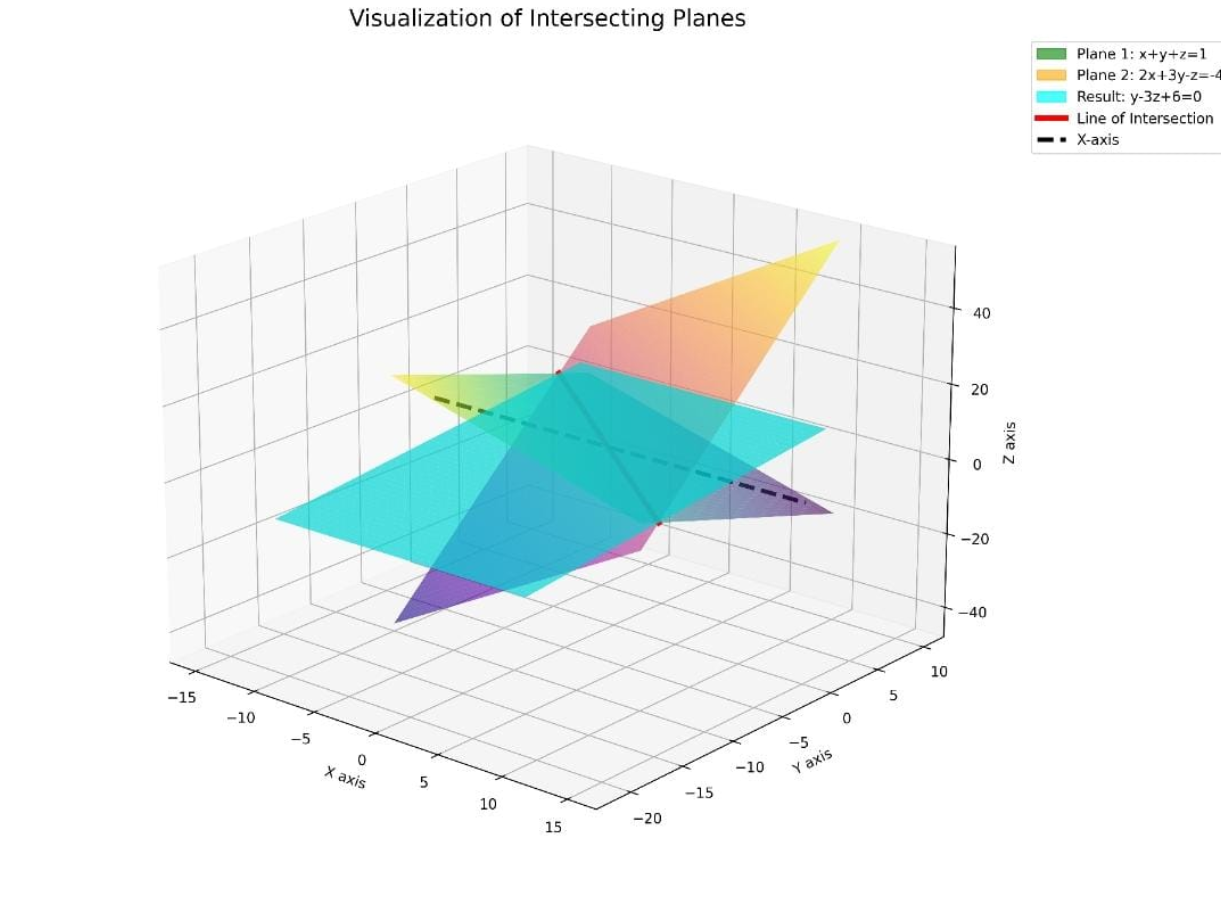
\includegraphics[width=0.75\columnwidth]{graph.png}
    \caption{Plot}
    \label{fig:placeholder}
\end{figure}
\end{frame}

\end{document}